% =====================================================================
%  Chapter 12 — The Data Problem
% =====================================================================

\chapter{The Data Problem}
\label{ch:data-problem}

Every quantitative claim in this book is downstream of a price series, and
the price series is where most published backtests quietly fail. This
chapter sets out the conventions the book's data layer uses, the four
failure modes it is built to survive, and what it deliberately does not
have.

\section{One source, cached, checksummed}

The book draws every price from a single source and holds nothing else.
This is a constraint, not an accident: a system that mixes sources must
reconcile their conventions at every join, and each reconciliation is a
place where a look-ahead can hide.

The pipeline has four stages. It requests a daily bar --- open, high, low,
close, adjusted close, volume --- for each fund over an explicit date
range, and it requests the dividend events separately. It writes each raw
response to disk, verbatim, with a SHA-256 checksum recorded in a
manifest. It validates what came back, and it refuses to proceed if the
validation fails. And it builds the panel from the cache, never from the
network, so that the numbers in the book are reproducible from the
repository alone.

The validation is not decorative. It checks that every series is finite
and non-empty; that the price is strictly positive; that the dates are
strictly increasing with no duplicates; that no gap between consecutive
observations exceeds ten calendar days, which catches both truncated
downloads and long suspensions; and that no single-day return exceeds a
plausibility bound, which catches unadjusted splits and bad vendor data.

\begin{takeaway}[The four integrity checks]
Finite values; strictly positive prices; strictly increasing dates with no
duplicates; no gap longer than ten days; and no implausible single-day
return. A fund that fails any of them does not enter the panel.
\end{takeaway}

\section{Why returns are rebuilt from components}

The vendor publishes an adjusted close: a price series with every
subsequent dividend and split applied backwards. Its ratios are total
returns, and its \emph{level} is meaningless. This book uses the adjusted
close only for ratios, and rebuilds the monthly total return from the raw
close and the dividend cash that was actually paid:

\begin{equation}
r_t = \left(1 + \frac{P_t - P_{t-1}}{P_{t-1}}\right)
      \left(1 + \frac{D_t}{P_{t-1}}\right) - 1,
\end{equation}
where \(P_t\) is the raw close at the end of month \(t\) and \(D_t\) is the
cash dividend paid during that month.

There are two reasons. The first is that the tax layer needs a genuine
transaction price, and the adjusted close is not one: its level has been
deflated by every dividend paid since. The second is that the vendor
applies its dividend factor on its own convention, which does not line up
exactly with the month in which the cash was paid, so the adjusted close
and the cash-based reconstruction disagree slightly.

That disagreement is measured rather than assumed. Across the panel, the
mean absolute difference between the two monthly return series is about
0.004 per cent --- three orders of magnitude smaller than any quantity the
book reports --- and the residual is entirely attributable to the
dividend-bucket convention. The two series are therefore used for two
different purposes: the cash-based one for everything the book computes,
and the vendor's as an independent check on it.

\section{The four ways a price series lies}

\subsection{Survivorship bias}

The universe is a list of funds that exist \emph{now}. A backtest that
assumes all of them were available throughout the sample is assuming that
no fund that was liquidated, merged or renamed away ever existed --- and
that every fund in the list was investable on every date it is used.

This book's defence is structural rather than statistical: every
allocation is made from the set of funds that have a price on the
formation date, so a fund that did not yet exist cannot be held, and a
fund that no longer exists cannot be held. The live window of each fund is
recorded and reported in Appendix A, and Chapter 13 shows what that window
looks like.

\subsection{Forward filling and the zero-return convention}

When a fund does not trade during a month --- a holiday, a market closure
in another jurisdiction, a suspension --- its last price is carried forward
and its return for that month is zero. Forward-filling the \emph{price}
rather than the return is the conservative choice: it cannot manufacture a
return, because a carried-forward price produces a zero return by
construction.

But it can manufacture a *risk* estimate, and this is the subtle point.
A fund that has not listed yet has no return at all, and treating its
missing months as zero returns would give it a realised volatility of
zero and a beta of zero --- which are not merely wrong numbers but
\emph{attractive-looking} wrong numbers, because a zero-volatility asset
is one a covariance-based optimiser would want to hold in quantity. The
book therefore masks the return series to missing before inception, and
computes covariances pairwise, so that a newly listed fund's own history
rather than an artefact of its non-existence determines its risk.

\subsection{The stale fundamentals problem}

A fund's assets under management, its expense ratio and its turnover are
published as of today, not as of the formation date. A backtest that uses
today's net assets to decide what to hold in 2004 is using a variable that
did not exist in the form it has now.

The book's defence is to use almost none of them. The expense ratio is
needed only for reporting, not for computation, because it is already
inside the return series. The net assets are needed only for reporting.
The turnover is not used at all. Every feature is computed from prices and
volume, both of which are contemporaneous and final.

\subsection{Revised macro data}

The most dangerous of all, and the one the book sidesteps entirely rather
than defending against. Macroeconomic series are revised, sometimes by
years, and the vintage of a revision is not usually available. A backtest
that uses a revised series will have used information that did not exist
at the formation date, and the error is invisible in the results.

The book's rule is that no feature may use a revised series. Where a
macro quantity is wanted --- a rate, a spread, a level of activity --- it
is \emph{proxied} from the price series itself. This is a real limitation
and it is not hidden: the feature set is deliberately price-based, which
means the book cannot claim that it has discovered anything about the
economy. What it can claim is that its inputs were all available on the
day they were used.

\begin{figure}[!htbp]
\centering
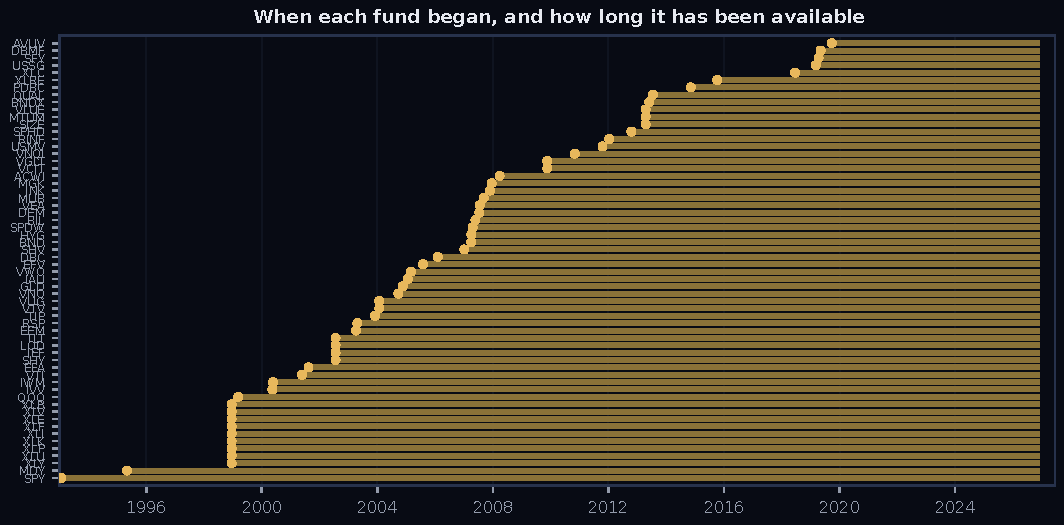
\includegraphics[width=\textwidth]{../figures/fig_live.pdf}
\caption{The live window of every fund in the universe. Each bar is the
period over which the fund had a price on the panel; the panel is not a
rectangle, and the system's allocation at any date is restricted to the
funds that had begun.}
\label{fig:live}
\end{figure}

\section{What the data layer cannot do}

The limits are worth stating as a list, because a system that pretends
otherwise is the thing this book is arguing against.

It cannot see valuation. There is no price-to-earnings, no price-to-book,
no cash-flow yield, because those require financial statements whose
filing dates and revisions are a second, separate data-quality problem.

It cannot see flows, sentiment or positioning. There is no volume-weighted
flow, no options data, no short interest.

It cannot see corporate events beyond the ones the vendor encodes in the
price series.

What it can do is make a narrow, precise claim: given the price and volume
history of a set of liquid exchange-traded funds, and nothing else, how
much can be estimated about the forward return of each of them, and how
confidently? That is a smaller question than the literature usually asks,
and it is the one this book answers.

\begin{keytakeaways}
\item One source, cached, checksummed, validated on five integrity checks,
and rebuilt from the cache rather than the network.
\item Monthly returns are rebuilt from raw price and dividend cash, because
the tax layer needs a real transaction price and because the vendor's
adjusted close uses a different dividend convention; the two series agree
to within 0.004 per cent a month.
\item Survivorship is handled structurally: only funds with a price on the
formation date can be held.
\item Missing months before inception are masked rather than zero-filled,
because a zero-volatility, zero-beta new listing is exactly the artefact
that makes a covariance optimiser want to buy it.
\item No revised macroeconomic series is used anywhere; macro quantities
are proxied from prices, and the feature set's limits are stated.
\end{keytakeaways}
